% $Id: notes.tex,v 1.31 2022/09/24 10:37:57 brandenb Exp $
%\documentclass{article}
\documentclass[twocolumn]{article}
\setlength{\textwidth}{160mm}
\setlength{\oddsidemargin}{-0mm}
\setlength{\textheight}{220mm}
\setlength{\topmargin}{-8mm}
\usepackage{graphicx,natbib,bm,url,color}
\graphicspath{{./fig/}{./png/}}
\thispagestyle{empty}
\input macros
\def\red{\textcolor{red}}
\def\blue{\textcolor{blue}}
\title{}
\author{}
\date{\today,~ $ $Revision: 1.31 $ $}
\begin{document}
%\maketitle

\section{Conservative formulation}

Solve
\begin{equation}
{T^{00}}_{,0}=-{T^{0i}}_{,i}
\end{equation}
\begin{equation}
{T^{i0}}_{,0}=-{T^{ij}}_{,j}
\end{equation}
where
\begin{equation}
E\equiv T^{00}={4\over3}\rho\gamma^2-{1\over3}\rho
={4\over3}\rho\gamma^2\left(1-1/4\gamma^2\right)
\end{equation}
\begin{equation}
T^{ij}={4\over3}\rho\gamma^2 u_i u_j+{1\over3}\rho\delta_{ij}
\label{hydroStress}
\end{equation}
Define
\begin{equation}
S_i\equiv T^{0i}=T^{i0}={4\over3}\rho\gamma^2 u_i
\end{equation}
So $\uu=\epsilon_u \SSS$, where
$\epsilon_u=3/(4\rho\gamma^2)=(1-1/4\gamma^2)/E$.
using $\uu^2=1-1/\gamma^2$,
\begin{equation}
r\equiv(T^{i0}/T^{00})^2={\gamma^4-\gamma^2\over(\gamma^2-1/4)^2}
\end{equation}
so
\begin{equation}
\gamma^4-\gamma^2-(\gamma^4-\gamma^2/2+1/16) r=0
\end{equation}
\begin{equation}
\gamma^4(1-r)-\gamma^2(1-r/2)-r/16=0
\end{equation}
\begin{equation}
\gamma^4-\gamma^2(1-r/2)/(1-r)-r/[16(1-r)]=0
\end{equation}
Solution for $\gamma^2$ is
\begin{equation}
\gamma^2={1-r/2\over2(1-r)}\pm\sqrt{
{(1-r/2)^2\over4(1-r)^2}+{r\over16(1-r)}}
\end{equation}
\begin{equation}
\gamma^2={1-r/2\over2(1-r)}\pm\sqrt{
{(1-r/2)^2\over4(1-r)^2}+{r-r^2\over16(1-r)^2}}
\end{equation}
\begin{equation}
\gamma^2={1\over2(1-r)}\left[(1-r/2)\pm\sqrt{
(1-r/2)^2+{r-r^2\over4}}\right]
\end{equation}
\begin{equation}
\gamma^2={1\over2(1-r)}\left[(1-r/2)\pm\sqrt{
1-r+r^2/4+{r-r^2\over4}}\right]
\end{equation}
\begin{equation}
\gamma^2={1\over2(1-r)}\left[(1-r/2)\pm\sqrt{
1-3r/4}\right]
\label{34eqn}
\end{equation}

\section{Keep $\cs^2$}

\begin{equation}
r\equiv(T^{i0}/T^{00})^2={\gamma^4-\gamma^2\over[\gamma^2-\cs^2/(1+\cs^2)]^2}
\end{equation}
\begin{equation}
\gamma^4-2\gamma^2\frac{\half-r\frac{\cs^2}{1+\cs^2}}{1-r}-\frac{r}{1-r}\left(\frac{\cs^2}{1+\cs^2}\right)^2=0
\end{equation}
\begin{equation}
\gamma^2=\frac{\half-r\frac{\cs^2}{1+\cs^2}}{1-r}
+\sqrt{\left(\frac{\half-r\frac{\cs^2}{1+\cs^2}}{1-r}\right)^2
+\frac{r}{1-r}\left(\frac{\cs^2}{1+\cs^2}\right)^2}
\end{equation}
\begin{equation}
\gamma^2=\frac{\half-r\frac{\cs^2}{1+\cs^2}}{1-r}
\left[1+\sqrt{1
+\left(\frac{1-r}{\half-r\frac{\cs^2}{1+\cs^2}}\right)^2
\frac{r}{1-r}\left(\frac{\cs^2}{1+\cs^2}\right)^2}\right]
\end{equation}
\begin{equation}
\gamma^2=\frac{\half-r\frac{\cs^2}{1+\cs^2}}{1-r}
\left[1+\sqrt{1
+\frac{(1-r)r}{\left(\half-r\frac{\cs^2}{1+\cs^2}\right)^2}
\left(\frac{\cs^2}{1+\cs^2}\right)^2}\right]
\end{equation}
\begin{equation}
\gamma^2=\frac{1}{1-r}
\left[\half-r\frac{\cs^2}{1+\cs^2}+\sqrt{\left(\half-r\frac{\cs^2}{1+\cs^2}\right)^2
+(1-r)r\left(\frac{\cs^2}{1+\cs^2}\right)^2}\right]
\end{equation}
\begin{equation}
\gamma^2=\frac{1}{1-r}
\left(\half-r\frac{\cs^2}{1+\cs^2}+\sqrt{\quarter-r\frac{\cs^2}{(1+\cs^2)^2}}\right)
\end{equation}
which agrees with \Eq{34eqn} for $\cs^2=1/3$ and $\gamma^2=1/(1-r)$ for $\cs^2=0$.
Here, $r$ plays the role of the square of a pseudo-velocity, so we could rename
$r\to r=v^2$, so then
\begin{equation}
\gamma^2=\frac{1}{1-v^2}
\left(\half-v^2\frac{\cs^2}{1+\cs^2}+\sqrt{\quarter-v^2\frac{\cs^2}{(1+\cs^2)^2}}\right)
\label{gamma2eqn}
\end{equation}

\begin{figure}[h!]\begin{center}
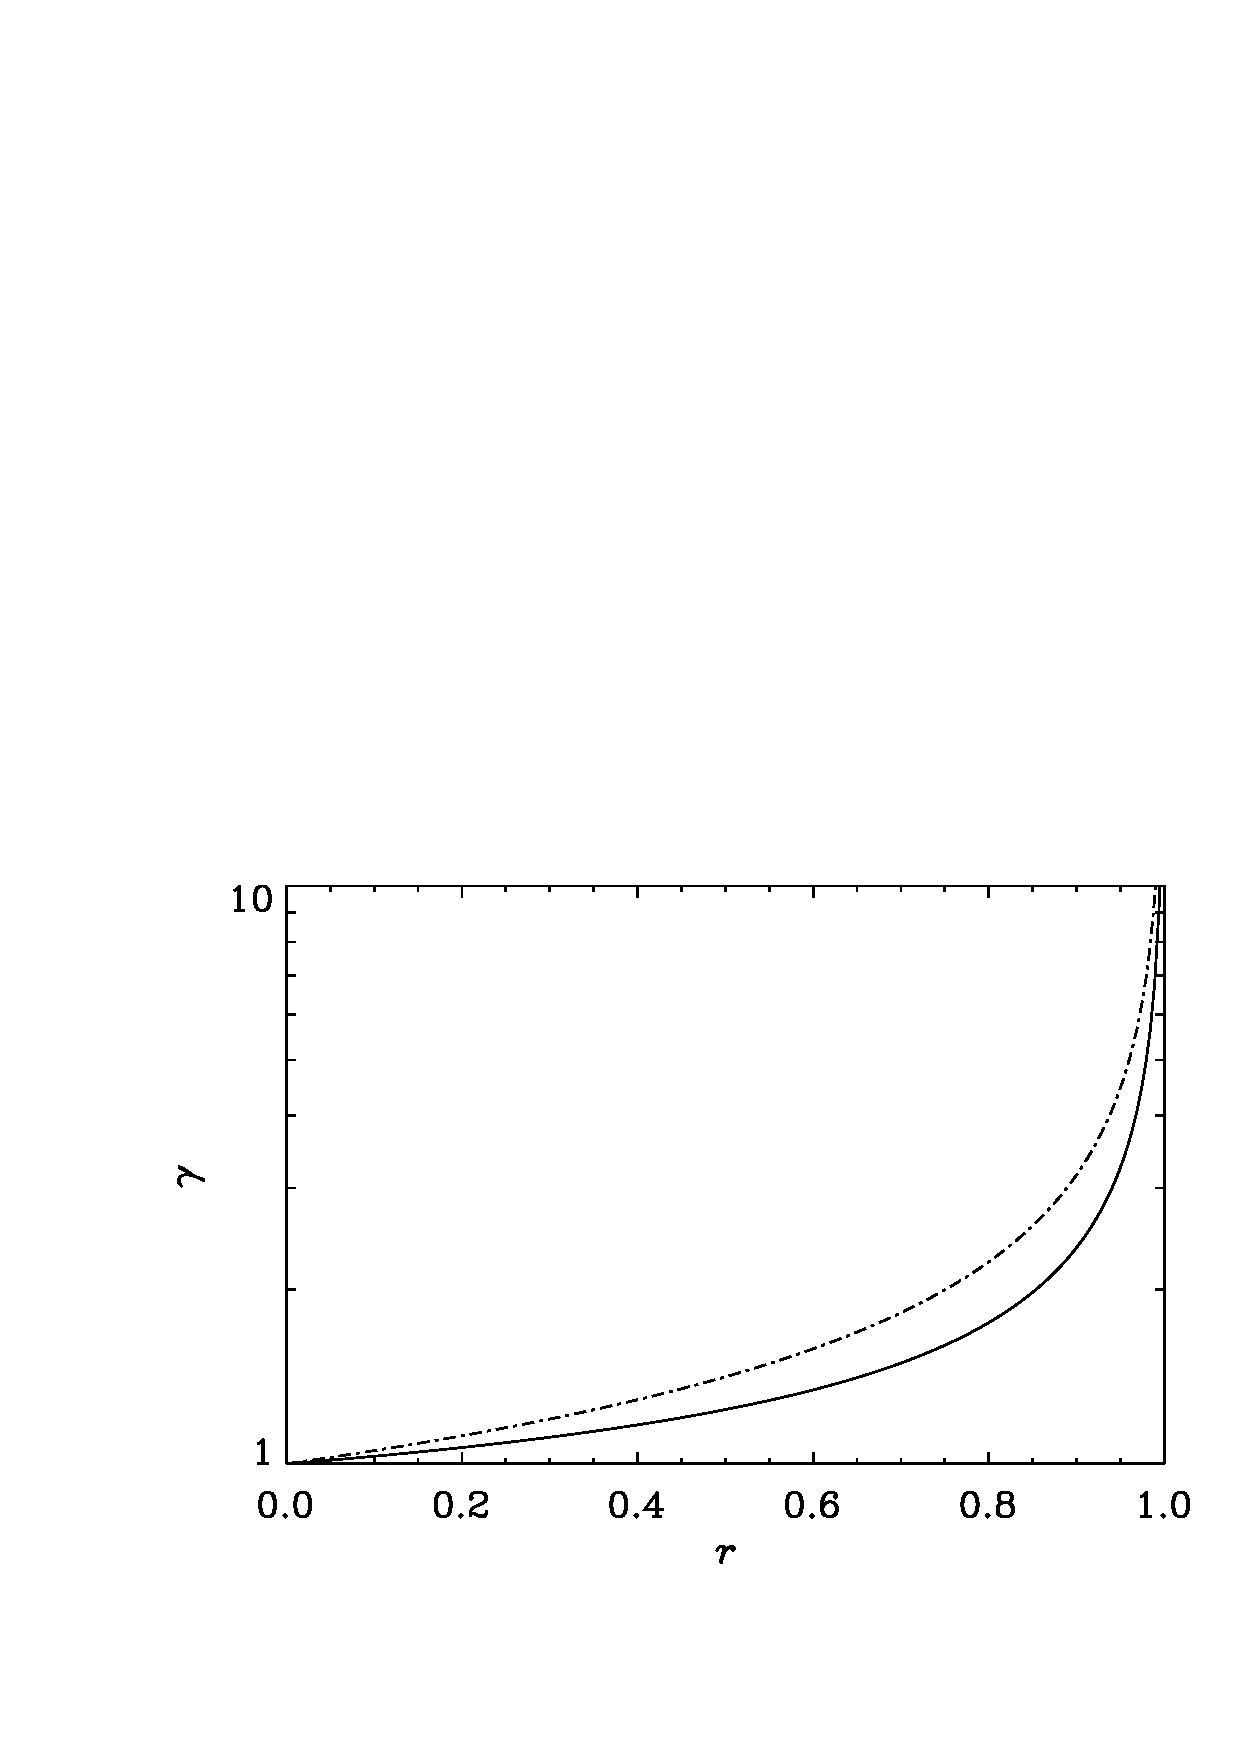
\includegraphics[width=\columnwidth]{p}
\end{center}\caption[]{
$\gamma$ versus $r$.
Solid line for $\cs^2=1/3$ and dashed-dotted line for $\cs=0$.
}\label{p}\end{figure}

\begin{figure*}[h!]\begin{center}
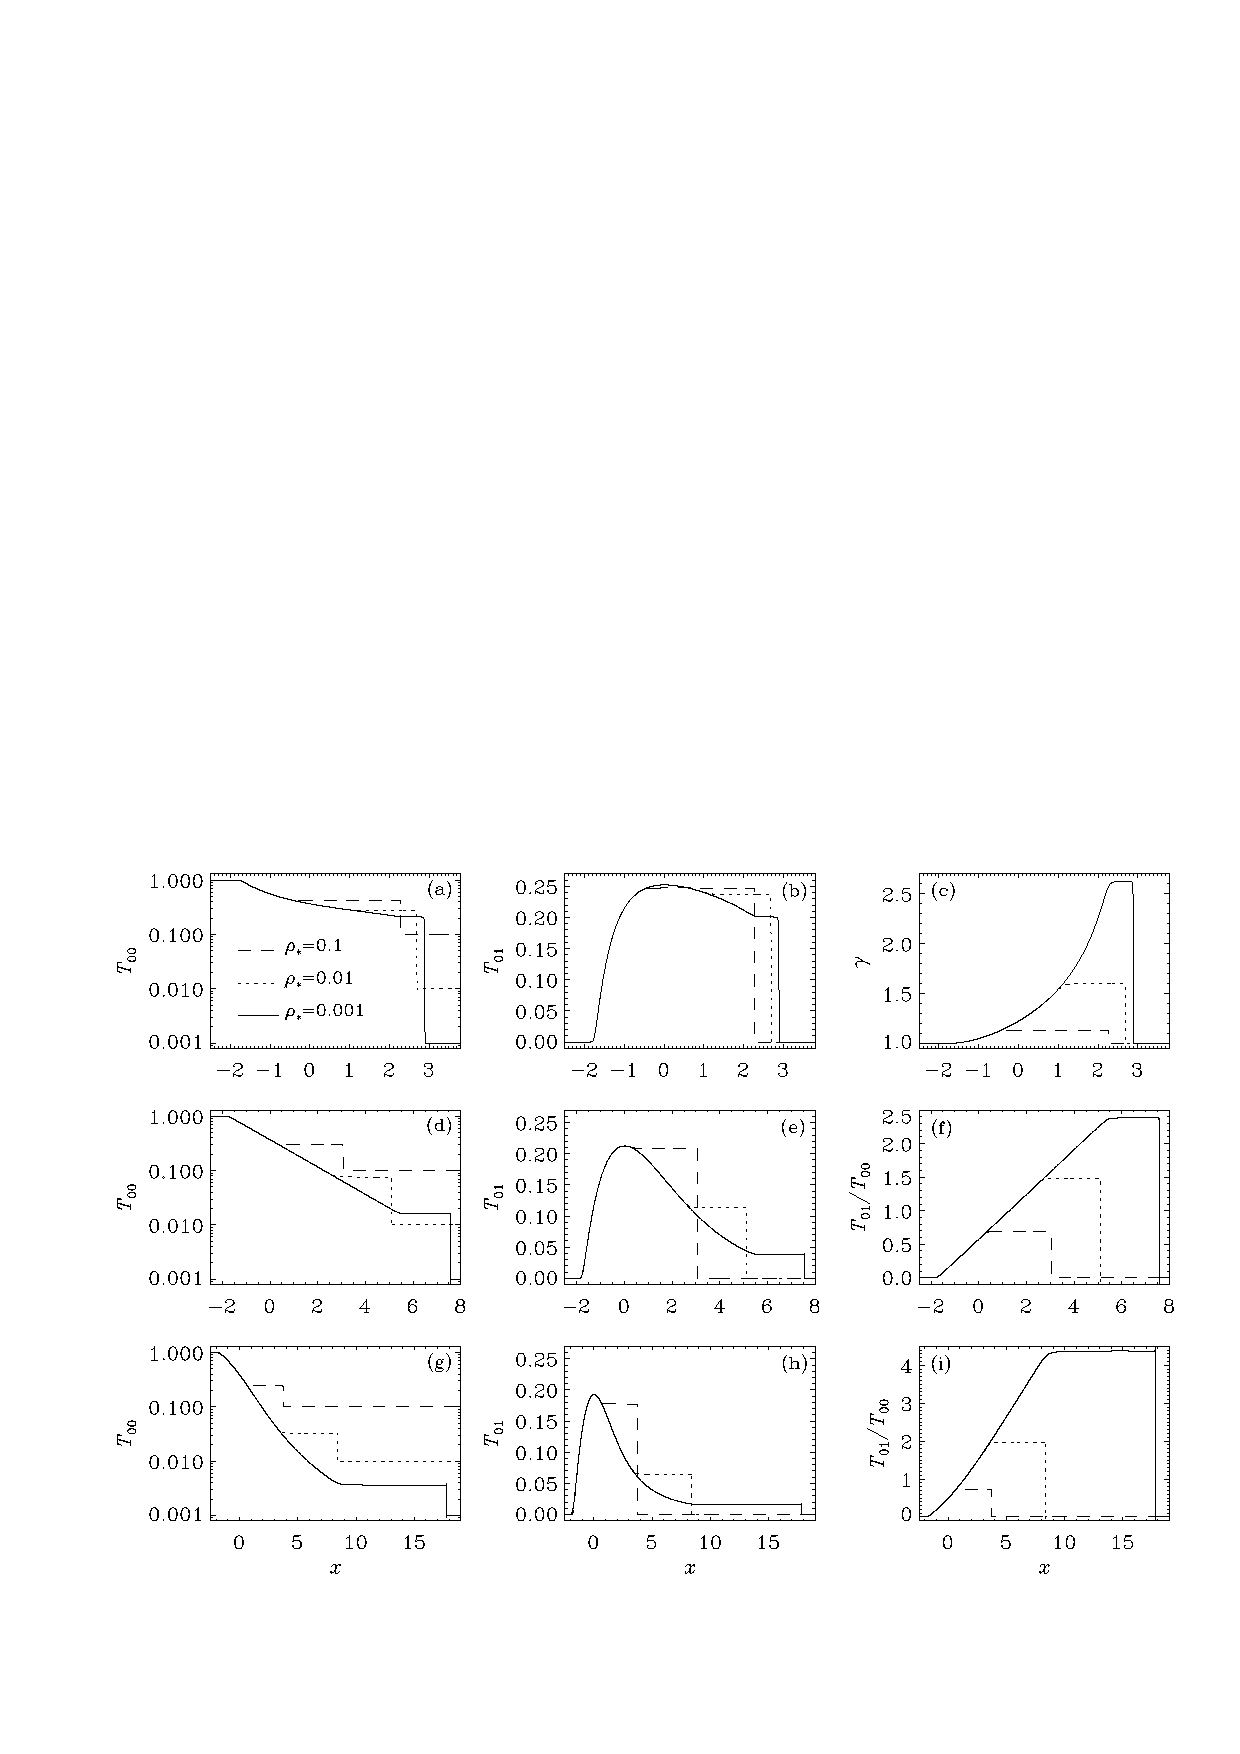
\includegraphics[width=\textwidth]{pcomp_shock}
\end{center}\caption[]{
Shock tube tests for (a)--(c) the relativistic case,
(d)--(f) the nonrelativistic case with isothermal equation of state, and
(g)--(i) the nonrelativistic case with ultrarelativistic equation of state.
}\label{pcomp_shock}\end{figure*}

\begin{table*}[htb]\caption{
Parameters used for the 1-D shock tube tests.
}\vspace{12pt}\centerline{\begin{tabular}{lccccccc}
Case          & $\delta x$ & $\delta t$ & $\nu$ & $\mu$ & $\gamma_{\max}$ & $u_{\max}$ \\
\hline
Relativistic  & $1.5\times10^{-3}$ & $2\times10^{-4}$ &$2\times10^{-4}$ &  $1\times10^{-4}$ & 1.13 & 0.47 \\% r4608b1_rel
              & $1.5\times10^{-3}$ & $2\times10^{-4}$ &$2\times10^{-4}$ &  $1\times10^{-4}$ & 1.60 & 0.78 \\% r4608c1_rel
              & $1.5\times10^{-3}$ & $2\times10^{-4}$ &$2\times10^{-4}$ &  $1\times10^{-4}$ & 2.63 & 0.92 \\% r4608d1_rel
\hline
Non-relativ.  & $1.5\times10^{-3}$ & $2\times10^{-4}$ &$5\times10^{-4}$ &  $1\times10^{-4}$ & 1.37 & 0.69 \\% r4608b1_nonrel
              & $1.6\times10^{-3}$ & $2\times10^{-4}$ &$5\times10^{-4}$ &  $2\times10^{-4}$ &  --  & 1.49 \\% r4608c1_nonrel
              & $2.2\times10^{-3}$ & $2\times10^{-4}$ &$5\times10^{-4}$ &  $2\times10^{-4}$ &  --  & 2.38 \\% r4608d1_nonrel
\hline
Relativ.\ EoS & $1.5\times10^{-3}$ & $2\times10^{-4}$ &$1\times10^{-3}$ &  $1\times10^{-4}$ & 1.20 & 0.55 \\% r4608b1_rel_eos
              & $2.7\times10^{-3}$ & $1\times10^{-4}$ &$2\times10^{-3}$ &  $1\times10^{-3}$ &  --  & 1.47 \\% r4608c1_rel_eos
              & $2.7\times10^{-3}$ & $1\times10^{-4}$ &$2\times10^{-3}$ &  $1\times10^{-3}$ &  --  & 3.28 \\% r8192d1_rel_eos
\label{Ttimescale}\end{tabular}}\end{table*}

%yutong/rel/2d
\begin{table}[htb]\caption{
Parameters used for 2-D turbulence tests.
$q_{\rm irro}=1$ (irrotational case).
}\vspace{12pt}\centerline{\begin{tabular}{lccccccc}
Run & $A$ & $\urms$ \\
\hline
A & 1.5 & 4.2771E-01 \\% r2048li
B & 1.2 & 3.6165E-01 \\% r2048lg
C & 1.0 & 3.1199E-01 \\% r2048lf
D & 0.9 & 2.8539E-01 \\% r2048le2
\label{Tdecay}\end{tabular}}\end{table}

\begin{figure}[h!]\begin{center}
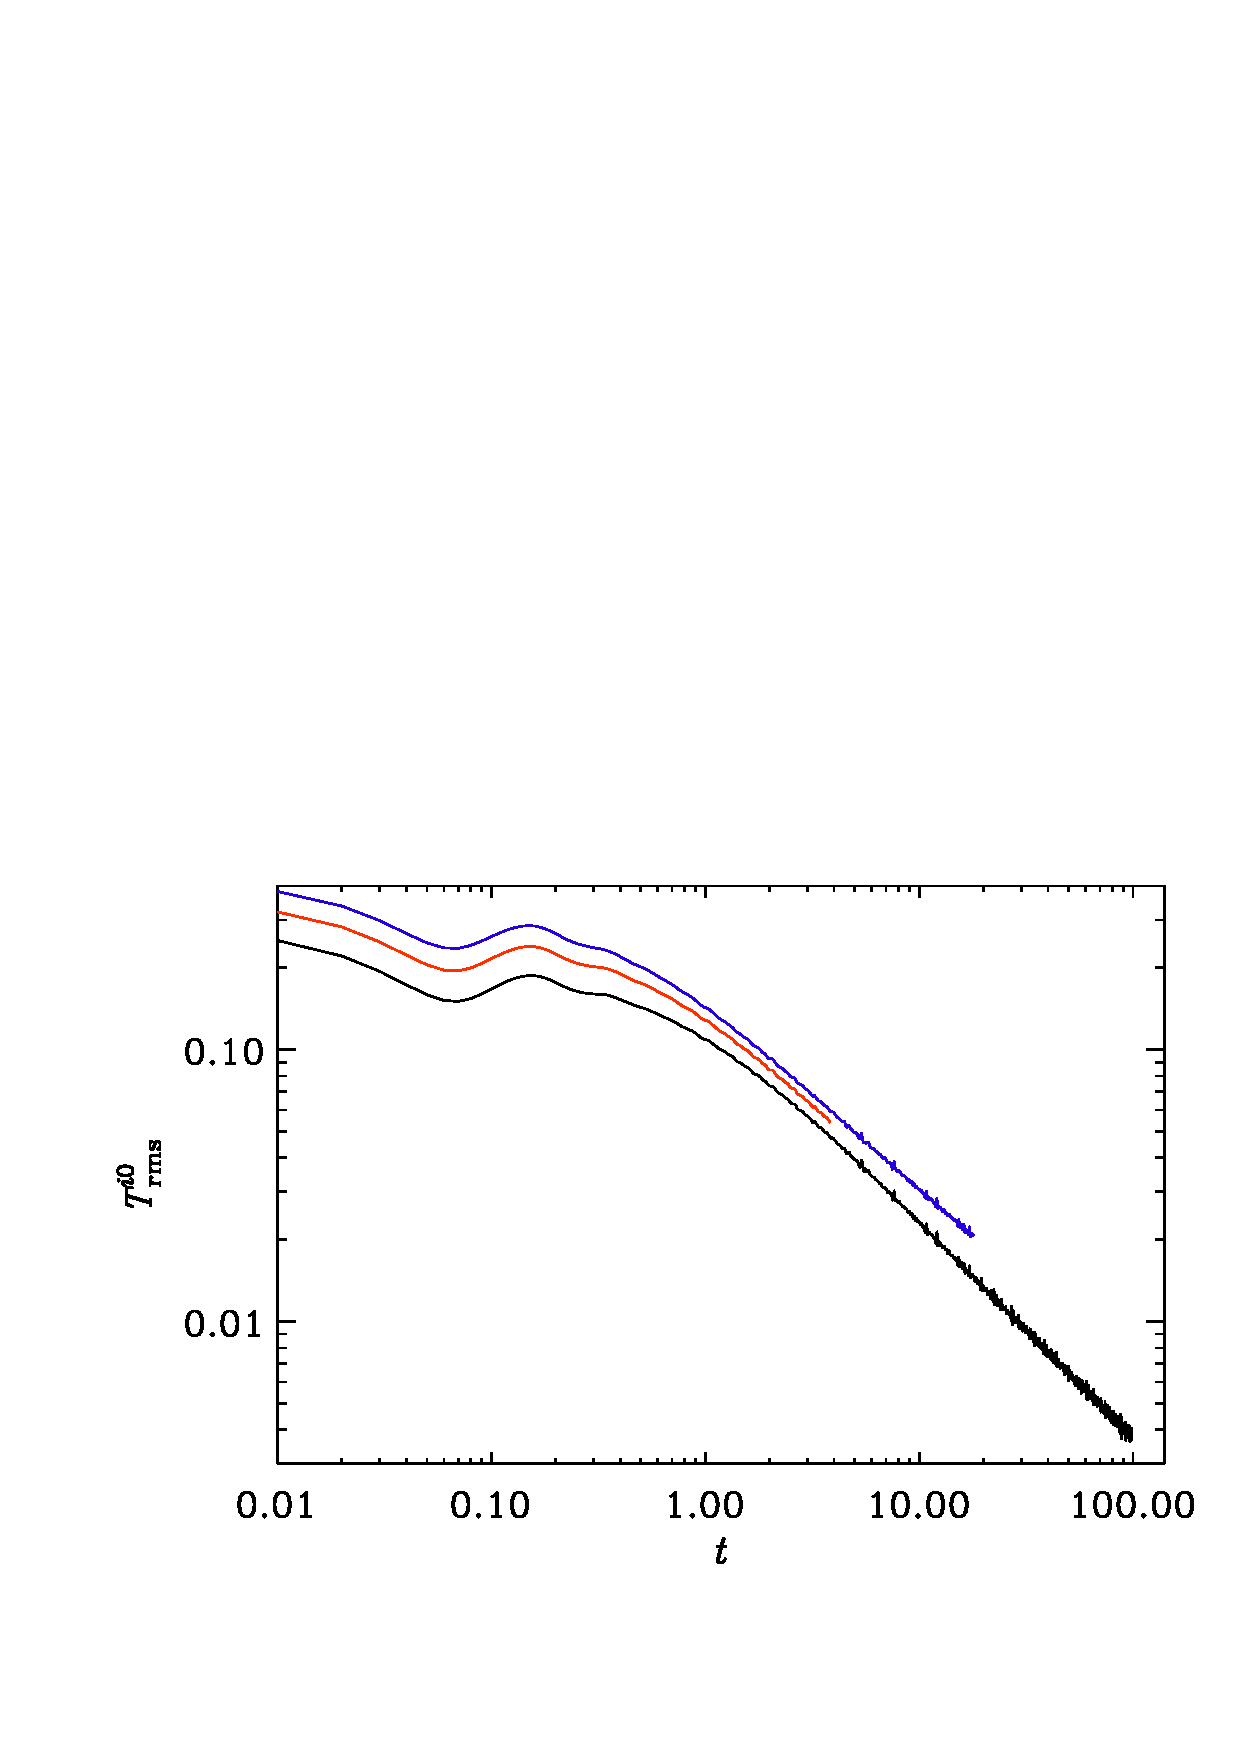
\includegraphics[width=\columnwidth]{pcomp}
\end{center}\caption[]{
2-D decaying turbulence for Runs A, B, and D.
}\label{pcomp}\end{figure}

\section{Computation of $T^{ij}$}

To compute $T^{ij}$, we use $T^{0i}$ and $T^{00}$.
We use \Eq{hydroStress} and $\rho/3=T^{00}/(4\gamma^2-1)$
to write
\begin{equation}
T^{ij}=\left(1-\frac{1}{4\gamma^2}\right)
\frac{T^{0i}T^{0j}}{T^{00}}
+\frac{T^{00}}{4\gamma^2-1}\delta_{ij}
\label{hydroStress2}
\end{equation}

\section{Magnetic runs}

In the momentum equation, the Reynolds/Maxwell tensor is
\begin{equation}
T^{ij}=\fourthird\rho\gamma^2 u_i u_j+\onethird\rho\delta_{ij}-B_iB_j+\half\BB^2\delta_{ij}
\end{equation}
We set $\EE=-\uu\times\BB+\eta\JJ$ and neglect term of
$O(\EE^2)\ll O(\BB^2)$.
Furthermore, the divergence of the magnetic part of $T^{ij}$ is just
$\JJ\times\BB$.
It is therefore convenient to solve
\begin{equation}
{T^{00}}_{,0}=-{T^{0i}}_{,i}
\end{equation}
\begin{equation}
{T^{i0}}_{,0}=-^{\rm H}{T^{ij}}_{,j}
\end{equation}
where $^{\rm H}{T^{ij}}$ is the hydro stress given by \Eq{hydroStress}.
The other components of the stress, ${T^{00}}$ and ${T^{i0}}$, however,
do contain the magnetic field.
In particular, we have
\begin{equation}
T^{00}=\fourthird\rho\gamma^2-\onethird\rho+\half\BB^2
\end{equation}
and
\begin{equation}
T^{0j}=\fourthird\rho\gamma^2 u_j+(\EE\times\BB)_j
\end{equation}
Here, ignoring the resistive term $\eta\JJ\times\BB$ for now, the Poynting
flux can also be written as
\begin{equation}
\EE\times\BB=(\BB^2\delta_{ij}-B_iB_j)u_j
\end{equation}
Therefore
\begin{equation}
T^{0i}=\left[\left(\fourthird\rho\gamma^2+\BB^2\right)\delta_{ij}-B_iB_j\right]u_j
\label{T0iTerm}
\end{equation}
\begin{equation}
\left(T^{0i}\right)^2=D^2\uu^2-\left(2D-\BB^2\right)(\uu\cdot\BB)^2
\end{equation}
where $D=\fourthird\rho\gamma^2+\BB^2$.
To calculate $r=v^2$, we use iteration:
\begin{equation}
v^2=\frac{\left(T^{0i}\right)^2+\left(2D-\BB^2\right)(\uu\cdot\BB)^2}
{\left(T^{00}-\half\BB^2\right)^2}
\end{equation}
or
\begin{equation}
v^2=\frac{\left(T^{0i}\right)^2+\left(\eightthird\rho\gamma^2+\BB^2\right)(\uu\cdot\BB)^2}
{\left(T^{00}-\half\BB^2\right)^2}
\label{v2mag}
\end{equation}
Assume for now $\uu\cdot\BB=0$, so
\begin{equation}
v^2=\frac{\left(T^{0i}\right)^2}
{\left(T^{00}-\half\BB^2\right)^2}
=\frac{D^2\uu^2}
{\left(T^{00}-\half\BB^2\right)^2}
\end{equation}
Thus, replacing $T^{00}-\half\BB^2=\fourthird\rho\gamma^2(1-1/4\gamma^2)$,
\begin{equation}
v^2=\frac{(\fourthird\rho\gamma^2+\BB^2)^2(1-1/\gamma^2)}
{(\fourthird\rho\gamma^2)^2(1-1/4\gamma^2)^2}
\end{equation}
so
\begin{equation}
v^2=\left(1+\frac{\BB^2}{\fourthird\rho\gamma^2}\right)^2
\frac{(1-1/\gamma^2)}
{(1-1/4\gamma^2)^2}
\end{equation}
or
\begin{equation}
v^2=\left(1+\frac{\BB^2}{\fourthird\rho\gamma^2}\right)^2
\frac{\gamma^2(\gamma^2-1)}
{(\gamma^2-1/4)^2}
\end{equation}
so in the magnetic case, where $v^2$ is given by \Eq{v2mag},
we have to replace in \Eq{gamma2eqn}
\begin{equation}
v^2\to v^2/[1+(\vA^{\rm nrel})^2]^2.
\end{equation}
where $(\vA^{\rm nrel})^2=\BB^2/(\fourthird\rho\gamma^2)$
is the pseudo Alfv\'en speed.
(It is also {\rm not} a non-relativistic one, because it contains $\gamma$.)

\section{Calculation of $u_i$ and hydro stress for $T^{ij}$}

Once we have $\gamma^2$, we can compute $\uu$ (here for, for Alfv\'en waves,
we have $\uu\cdot\BB=0$) using \Eq{T0iTerm},
\begin{equation}
u_i=\frac{T^{0i}}{\fourthird\rho\gamma^2+\BB^2}
\end{equation}
or, in terms of $T^{00}$, using
\begin{equation}
\fourthird\rho\gamma^2=\frac{T^{00}-\half\BB^2}{1-\frac{1}{4\gamma^2}},
\end{equation}
we have
\begin{equation}
u_i=\frac{T^{0i}}{\displaystyle{\frac{T^{00}-\half\BB^2}{1-1/4\gamma^2}}+\BB^2}
\end{equation}
which is the expression used currently in the code.
By expanding it, it can also be written as
\begin{equation}
u_i=\frac{T^{0i}(1-1/4\gamma^2)}{T^{00}-\half\BB^2+(1-1/4\gamma^2)\BB^2}
\end{equation}
to get
\begin{equation}
u_i=\frac{T^{0i}(1-1/4\gamma^2)}{T^{00}+(1-1/2\gamma^2)\BB^2/2}
\end{equation}

To compute $^{\rm H}T^{ij}$, we again use $T^{0i}$ and $T^{00}$.
We use \Eq{hydroStress} and $\rho/3=(T^{00}-\half\BB^2)/(4\gamma^2-1)$
to write
\begin{equation}
T^{ij}=\frac{T^{0i}T^{0j}}{(T^{00}-\half\BB^2)/(1-1/4\gamma^2)+\BB^2}
+\frac{T^{00}-\half\BB^2}{4\gamma^2-1}\delta_{ij}
\end{equation}
where
\begin{equation}
\fourthird\rho\gamma^2=
\frac{T^{00}-\half\BB^2}{1-1/4\gamma^2}
\end{equation}
and
\begin{equation}
\onethird\rho=
\frac{T^{00}-\half\BB^2}{4\gamma^2-1}
\end{equation}
and therefore more compactly
\begin{equation}
T^{ij}=\frac{T^{0i}T^{0j}}{\fourthird\rho\gamma^2+\BB^2}
+\onethird\rho\delta_{ij}
\label{hydroStress3}
\end{equation}
In terms of $\cs$ etc, we have
\begin{equation}
\rho=\frac{T^{00}-\half\BB^2}{(1+\cs^2)\gamma^2-\cs^2}
\end{equation}
and
\begin{equation}
\frac{1}{1-1/4\gamma^2}\to
\frac{1}{1-\cs^2/[\gamma^2(1+\cs^2)]}
\end{equation}
or
\begin{equation}
\frac{1}{1-1/4\gamma^2}\to
\frac{(1+\cs^2)\gamma^2}{(1+\cs^2)\gamma^2-\cs^2}
\end{equation}

%r e f
%\begin{thebibliography}{}

%\bibitem[Biskamp \& M\"uller(1999)]{BM99}
%Biskamp, D., \& M\"uller, W.-C.\yprl{1999}{83}{2195}

%\end{thebibliography}

%\vfill\bigskip\noindent\tiny\begin{verbatim}
%$Header: /var/cvs/brandenb/tex/yutong/rel/notes.tex,v 1.31 2022/09/24 10:37:57 brandenb Exp $
%\end{verbatim}

\end{document}
